\begin{frame}{}
	
	\textbf{What is the parareal method ?}
	
	\begin{enumerate}[\textbullet]
		\item parallel-in-time integration method, introduced in 2001 by Lions, Maday and Turinici~\cite{partie2_ref1}
		\item computes the numerical solution for multiple time steps in parallel
		\item categorized as a parallel-across-the-steps method 
	\end{enumerate}

	\textbf{Objectives for parareal method}

	\begin{enumerate}[\textbullet]
		\item Implement the parareal method in C++ and :
		\begin{itemize}
			\item Test the method (with oscillator)
			\item Check convergence and stability results
			\item Check speed-up and efficiency 
		\end{itemize}
		\item Implement the resolution of the heat equation in C++ with Feel++ \\
		$\Rightarrow \quad $ Implement the resolution of the Laplace equation in C++ with Feel++ \\
		\item Use the previous implementation of the heat equation with the parareal method
		\item Check the convergences/accuracies of the method
	\end{enumerate}
	
\end{frame}


\subsection{Theory}

\begin{frame}{Generalities of the parareal method}
	Time decomposition :
	\begin{enumerate}[\textbullet]
		\item $[t_0,T]=[t_0,t_1]\cup\dots\cup[t_{P-1},t_P]$ with $t_P=T$ and $P=$ number of processes
	\end{enumerate}

	\; \\

	\begin{minipage}{\linewidth}
		Notations :
		\begin{enumerate}[\textbullet]
			\item $F$ : high accuracy integrator, \quad $\Delta t_F$ : time step \\
			$G$ : low accuracy integrator, \quad $\Delta t_G$ : coarse time step
			\item $U_j^k, j\in\{0,\dots,P\}$ : initial point at time $t_j$ and at iteration $k$.
		\end{enumerate}
	\end{minipage} \\
	\begin{enumerate}[\textbullet]
		\item $F(U_{j-1}^k), j\in\{1,\dots,P\}$ : value of the fine integrator at $t_j$ starting by $U_{j-1}^k$ \\
		(resp. $G(U_{j-1}^k)$) \\
		$F$ and $G$ are Runge Kutta of order 4 
		\begin{minipage}{\linewidth}
			\centering
			\qquad \qquad \qquad \qquad \qquad \qquad \qquad
			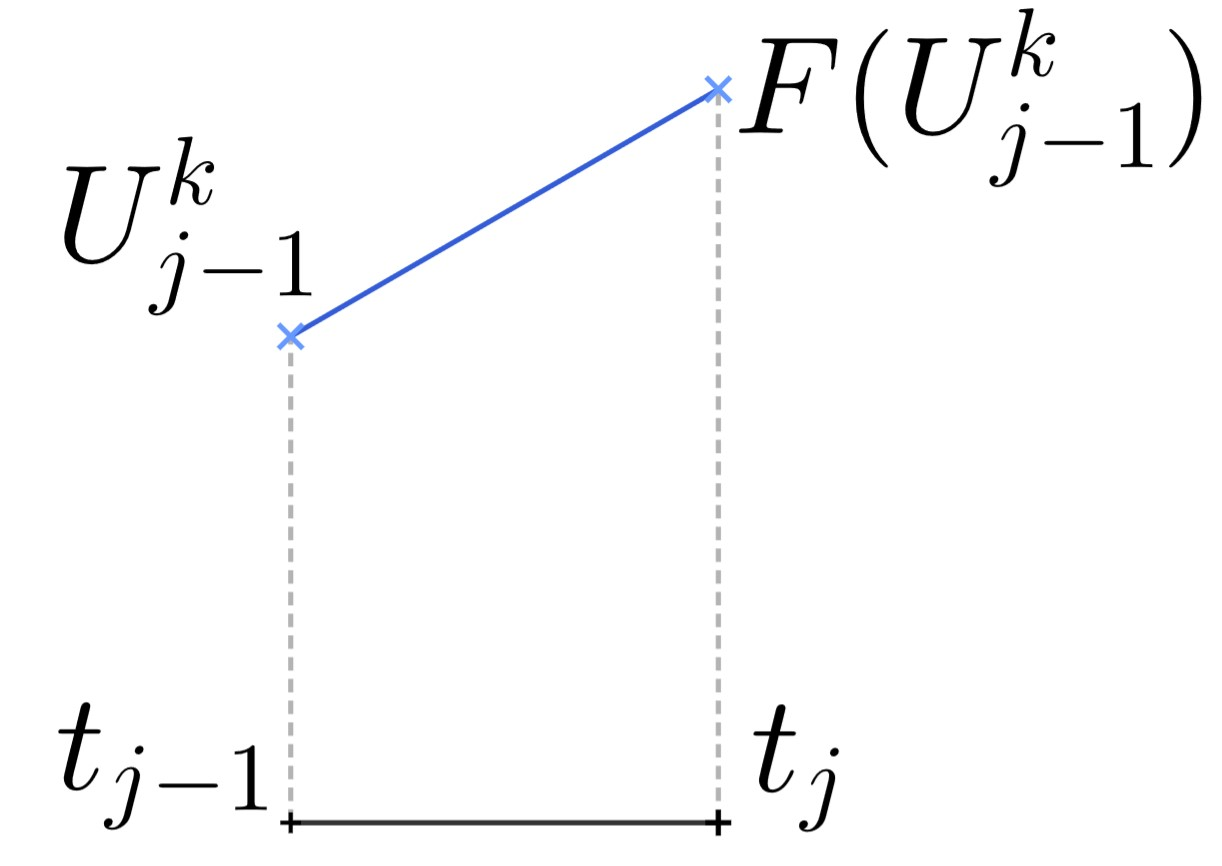
\includegraphics[width=0.3\linewidth]{images/parareal/explane_F.jpg}
		\end{minipage}
	\end{enumerate}
	
	
\end{frame}

\begin{frame}[allowframebreaks]{Explanation of the parareal method}
	\begin{figure}
		\centering
		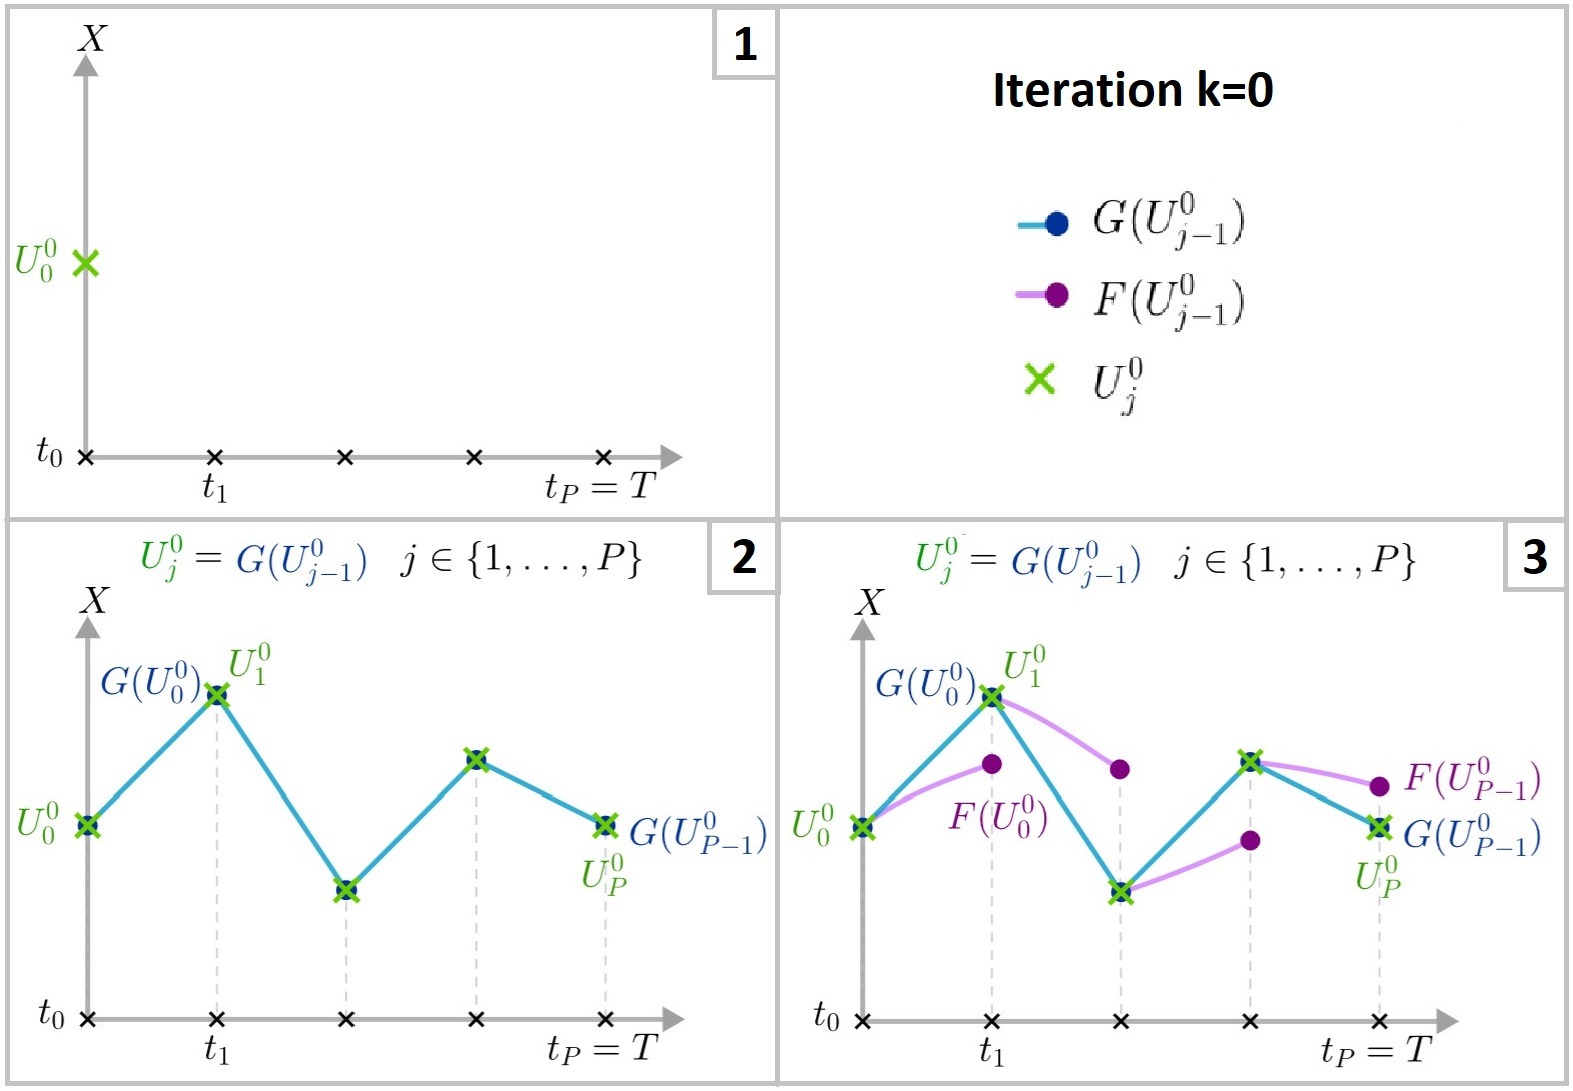
\includegraphics[width=0.6\linewidth]{images/parareal/parareal_k0.jpg}
		\caption{Explanation of the parareal method at iteration $k=0$ (step 1 to 3)}
	\end{figure}
	\begin{figure}
		\centering
		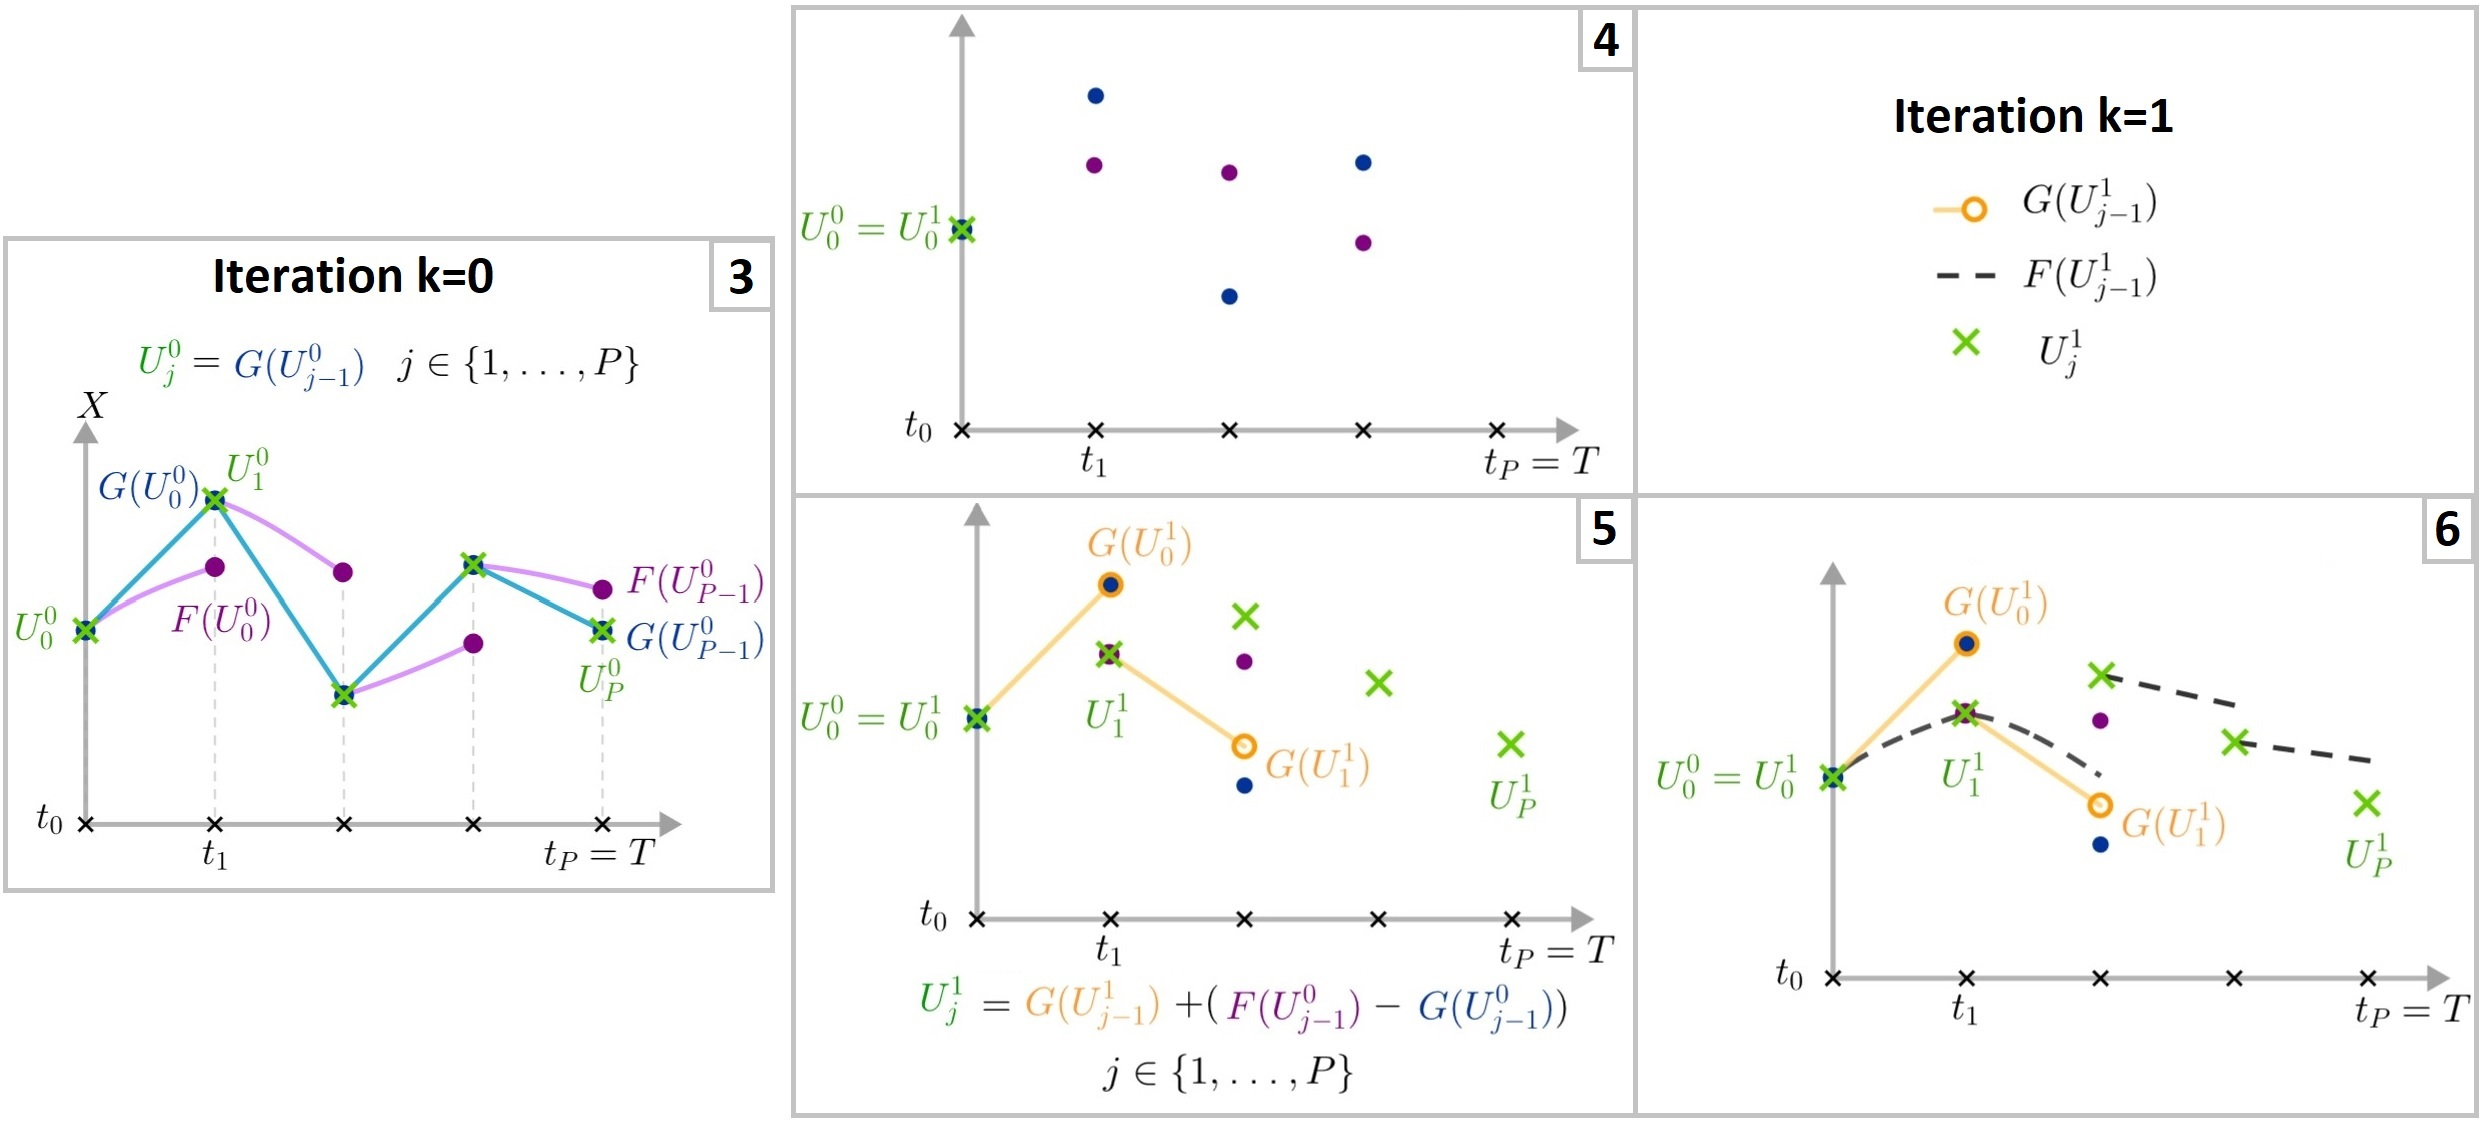
\includegraphics[width=0.9\linewidth]{images/parareal/parareal_k1.jpg}
		\caption{Explanation of the parareal method at iteration $k=1$ (step 4 to 6)}
	\end{figure}
	\small
	We have at iteration $k$ : \qquad	$U_j^k=G(U_{j-1}^k)+(F(U_{j-1}^{k-1})-G(U_{j-1}^{k-1}))$
\end{frame}

\begin{frame}[allowframebreaks]{Algorithm}
	 \begin{figure}
	 	\centering
	 	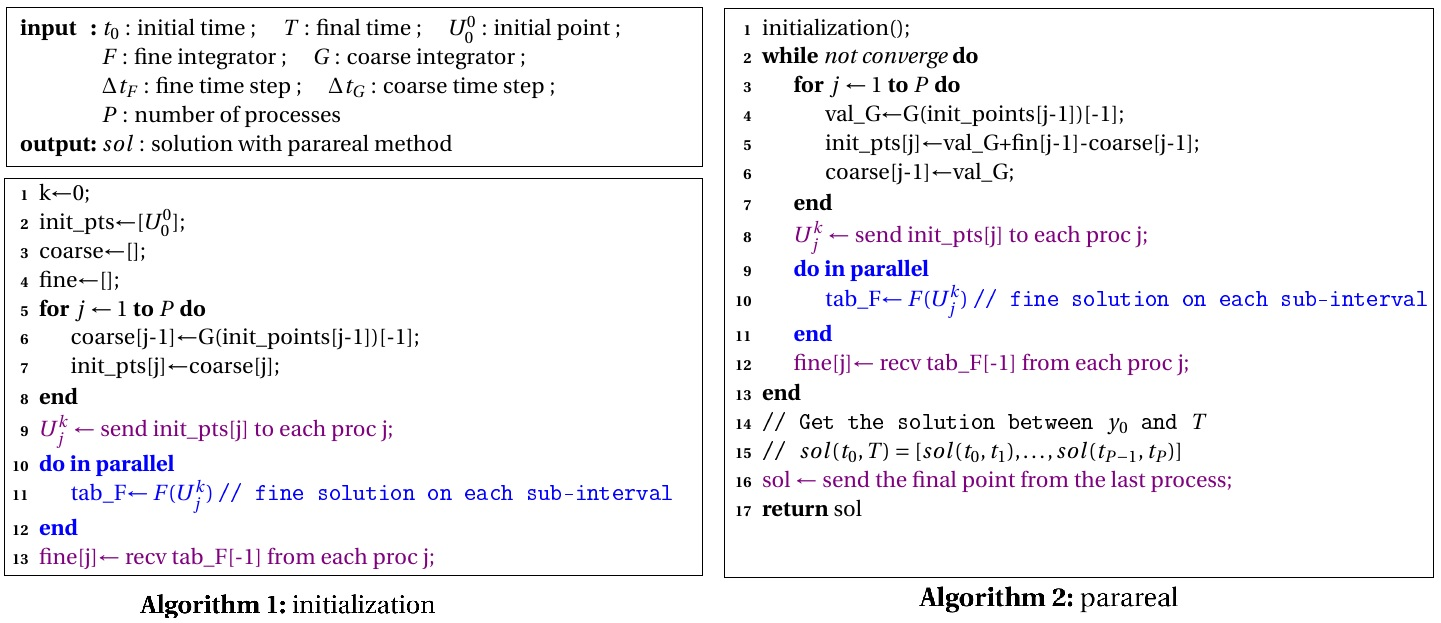
\includegraphics[width=\linewidth]{images/parareal/algorithm.jpg}
	 	\caption{Algorithm for the parareal method}
	 \end{figure}
\end{frame}

\begin{frame}{Order of the parareal method}
	The parareal method is of order k if there is a constant $c_k$ such that :
	\begin{equation*}
		\forall j\in\{0,\dots,P-1\} \qquad \mathcal{E}(j,k)\le c_k(\Delta t_G)^k
	\end{equation*}
	with
	$$\mathcal{E}(j,k)=|U_j^k-U_{ex}(t_j)|+\max_{t\in[t_j,t_{j+1}]}|U_k(t)-U_{ex}(t)|$$
	\begin{figure}
		\centering
		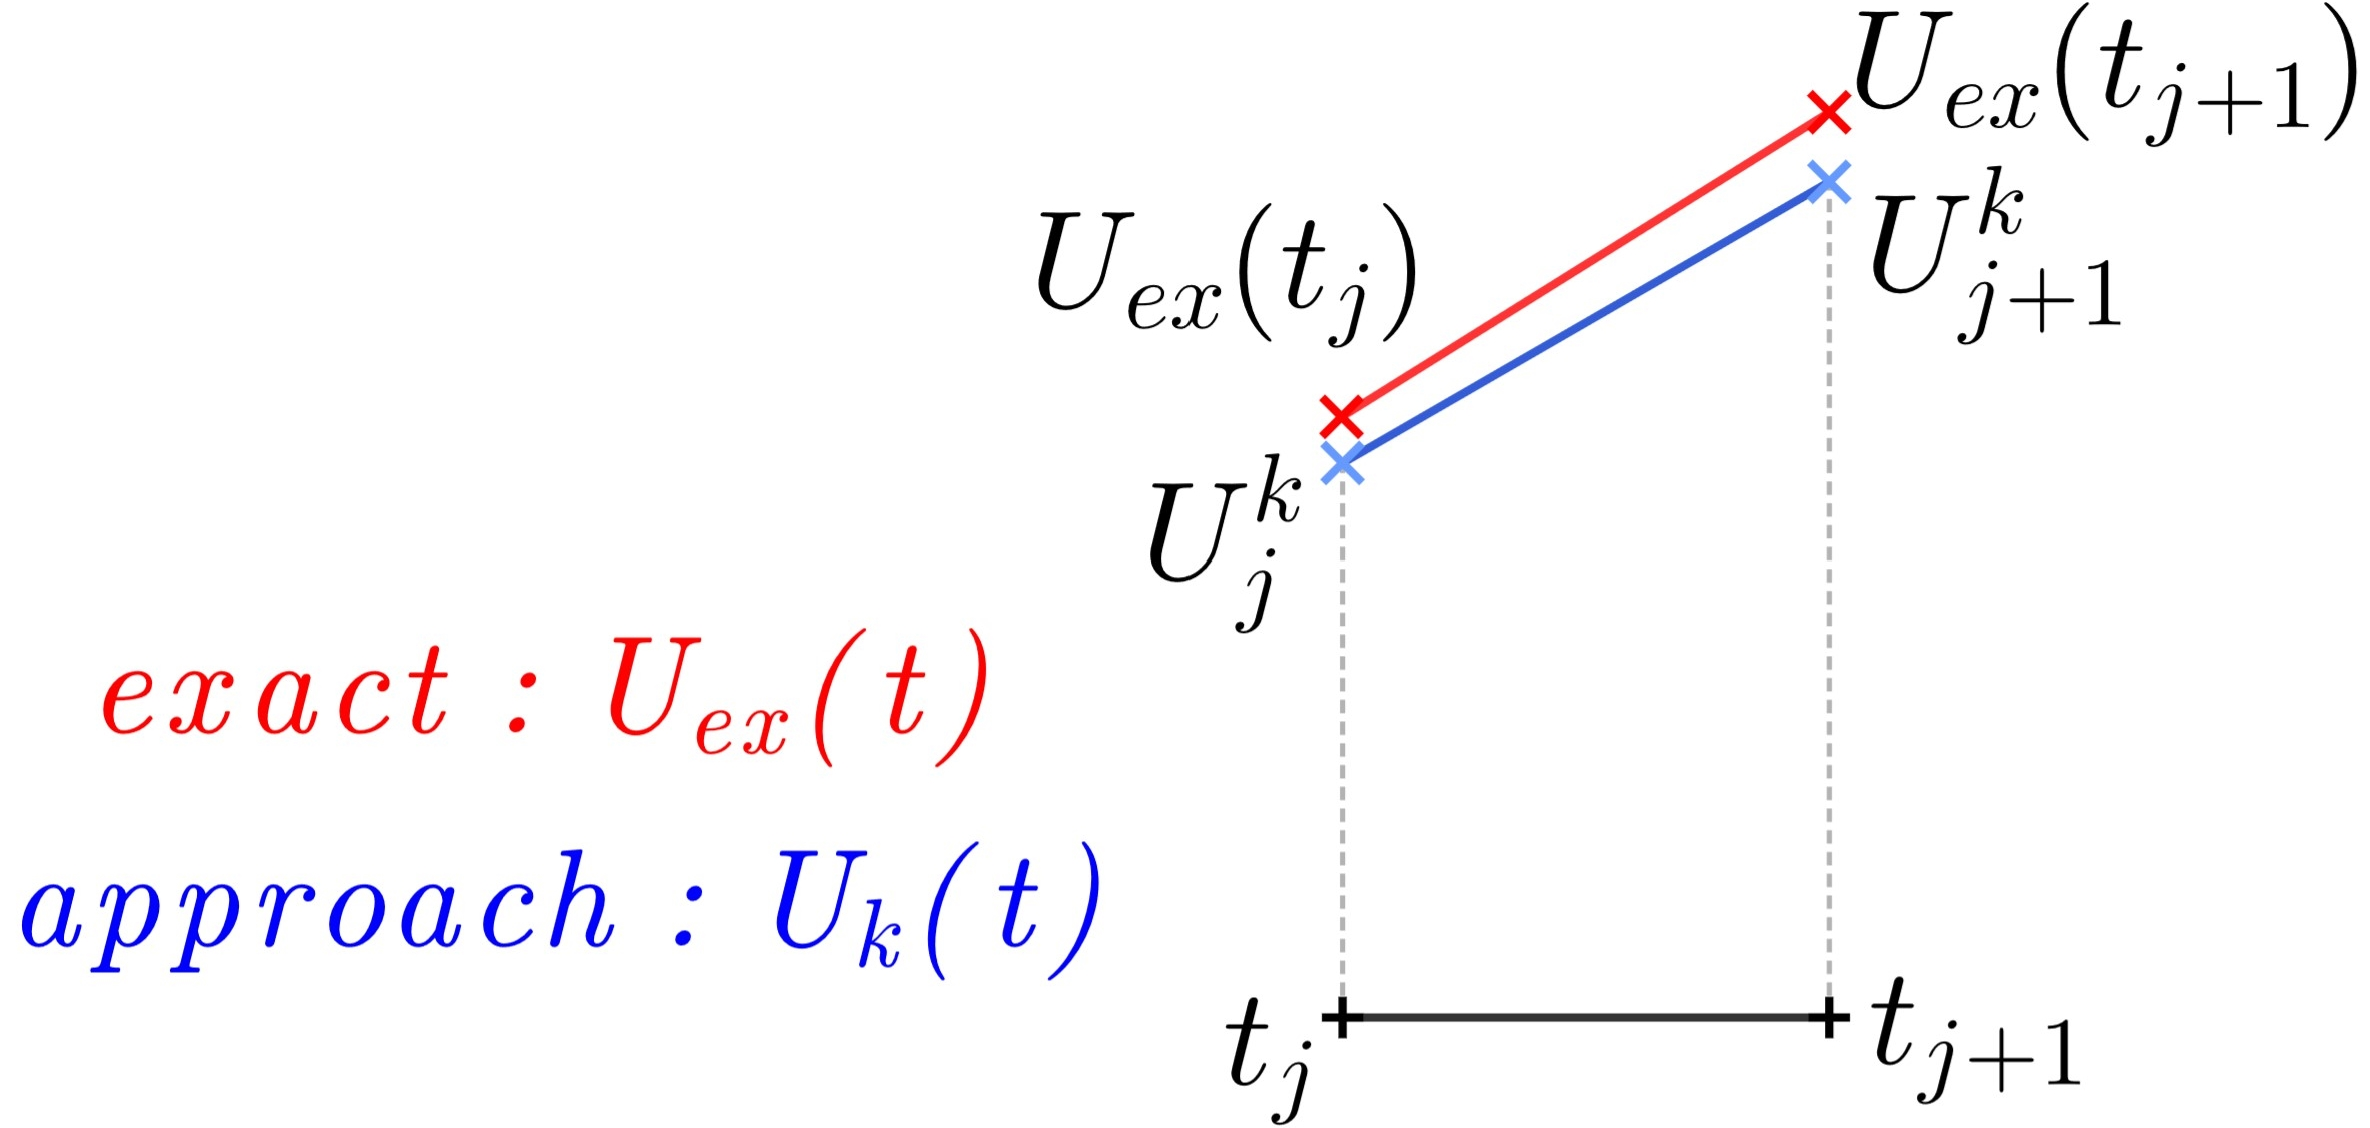
\includegraphics[width=0.62\linewidth]{images/parareal/explane_order.jpg}
		\caption{Explanation of the order property}
	\end{figure}
\end{frame}

\section{Application in Python and C++}

\begin{frame}{Example with the Lorenz system}
	\centering
	$\sigma=10, \quad b=\frac{8}{3}, \quad r=28, \quad X_0=(5,5,5), \quad t_0=0, \quad T=20$
	$P=4,\quad \Delta t_G=0.1, \quad \Delta t_F=0.01$
	\begin{figure}
		\centering
		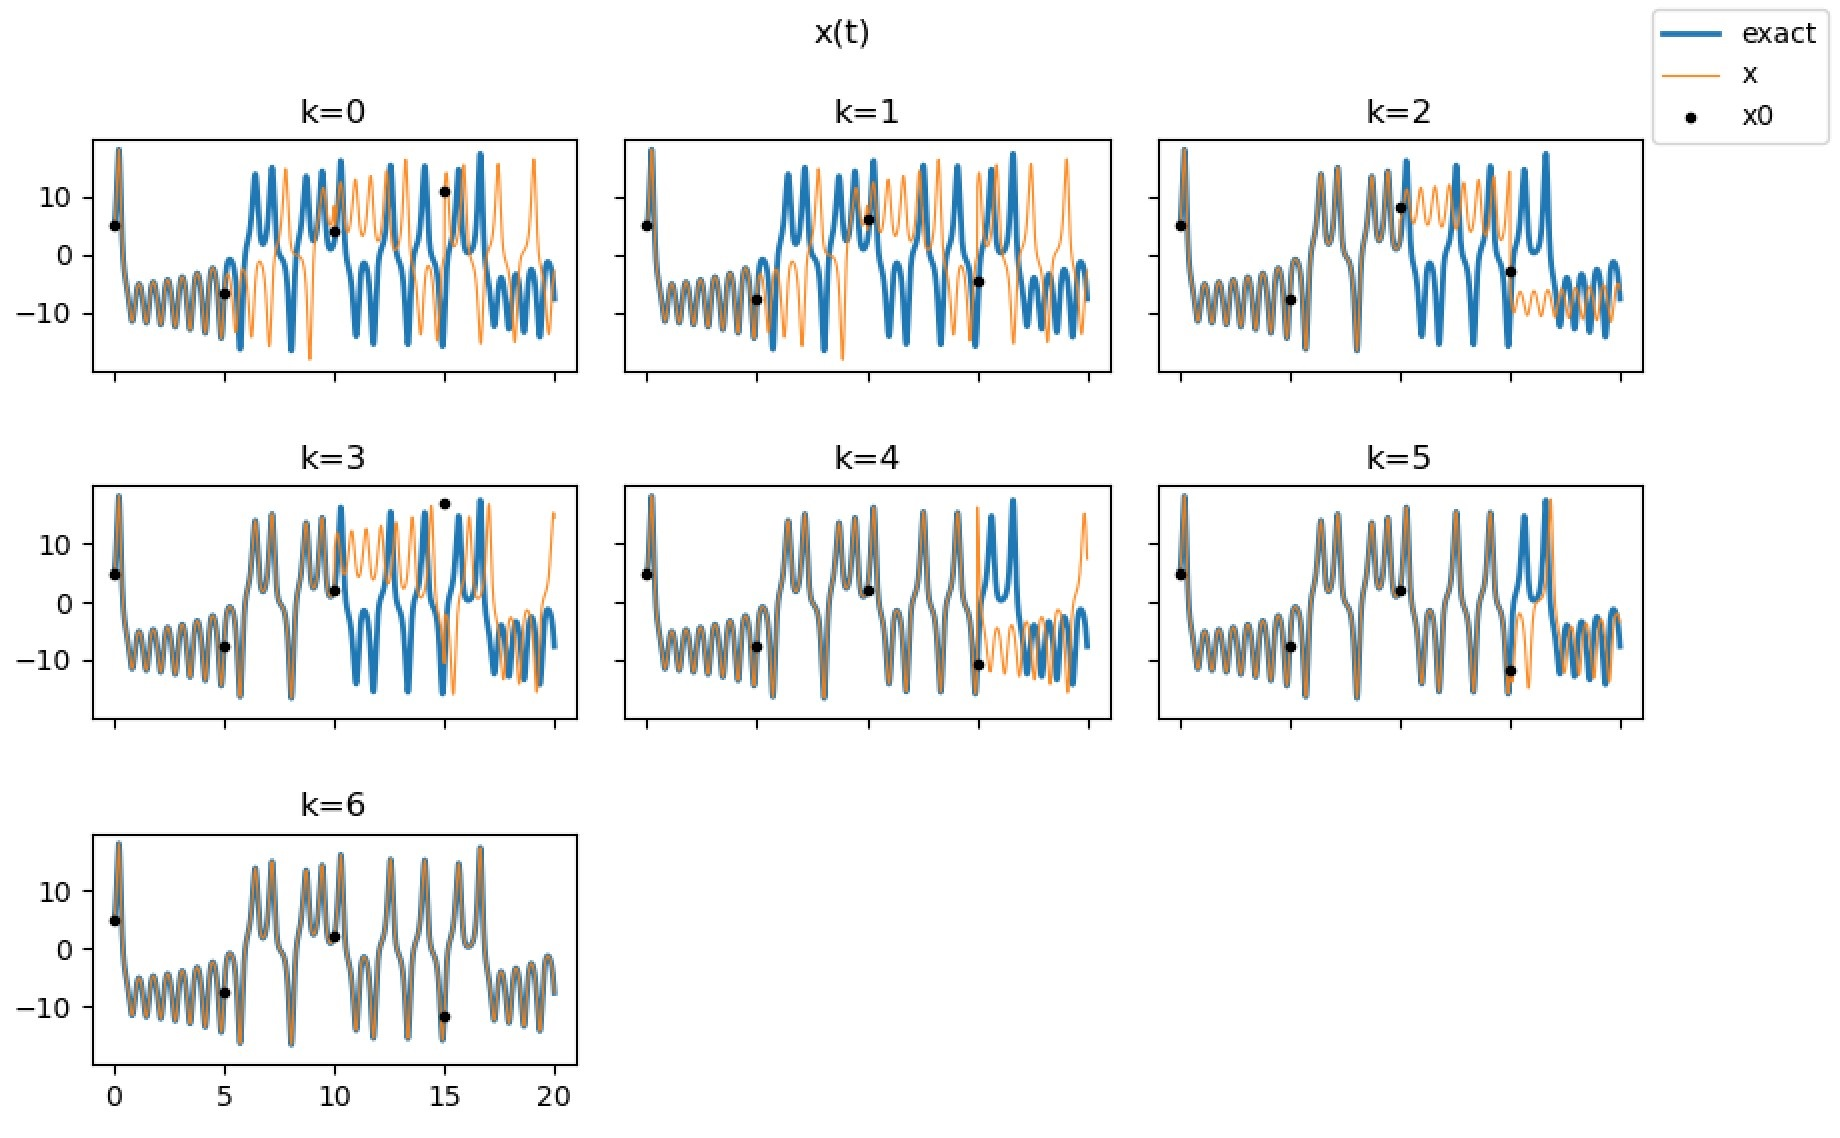
\includegraphics[width=0.8\linewidth]{"images/parareal/lorenz_4p.jpg"}
		\caption{Solution of the Lorenz system with C++ at each iteration}
	\end{figure}
\end{frame}

\begin{frame}{Speed-up for the Lorenz system}
	\begin{figure}
		\centering
		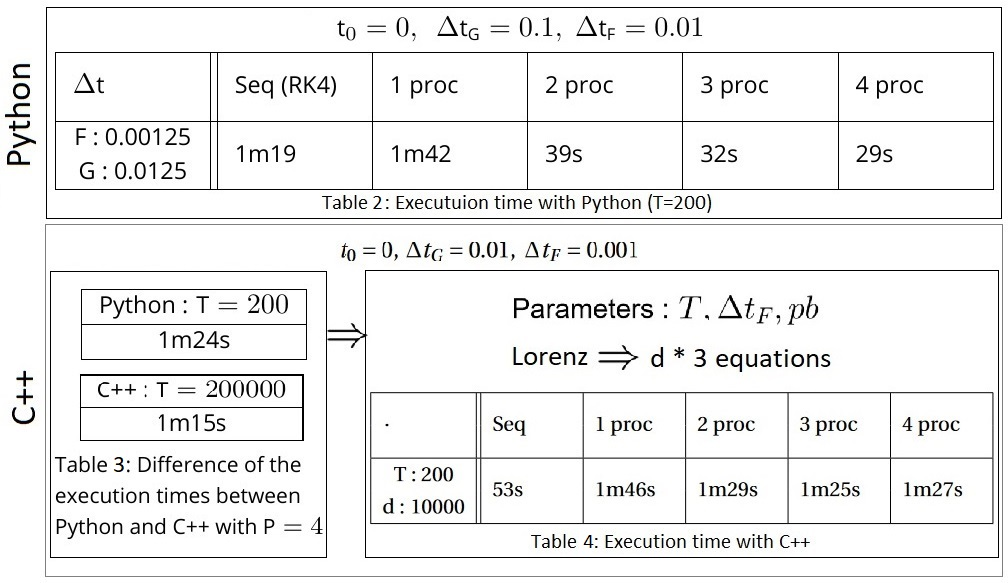
\includegraphics[width=0.9\linewidth]{"images/parareal/speedup_lorenz.jpg"}
	\end{figure}
\end{frame}

\begin{frame}{Incorrect results for the Lorenz System}
	\centering
	$\sigma=10, \; b=\frac{8}{3}, \; r=28, \; X_0=(5,5,5), \; t_0=0, \; \Delta t_G=0.1, \; \Delta t_F=0.01$
	\begin{figure}
		\centering
		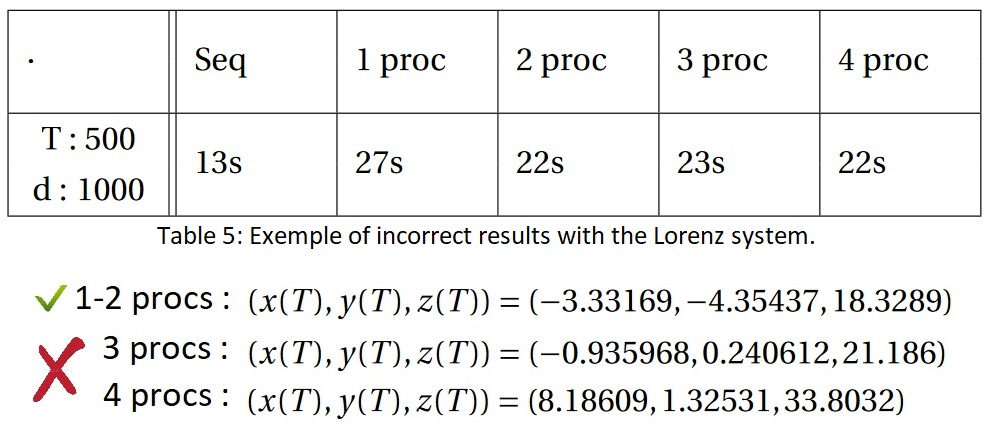
\includegraphics[width=0.9\linewidth]{"images/parareal/incorrect_results.jpg"}
	\end{figure}
\end{frame}


\begin{frame}{Example for the Harmonic oscillator}
	
	$$P=3, \quad x(0)=0,\quad v(0)=1, \quad\omega_0=5, \quad x_0=\frac{-1}{5}, \quad \phi_0=\frac{\pi}{2}$$
	
	\begin{minipage}{0.45\linewidth}
		\begin{figure}
			\centering
			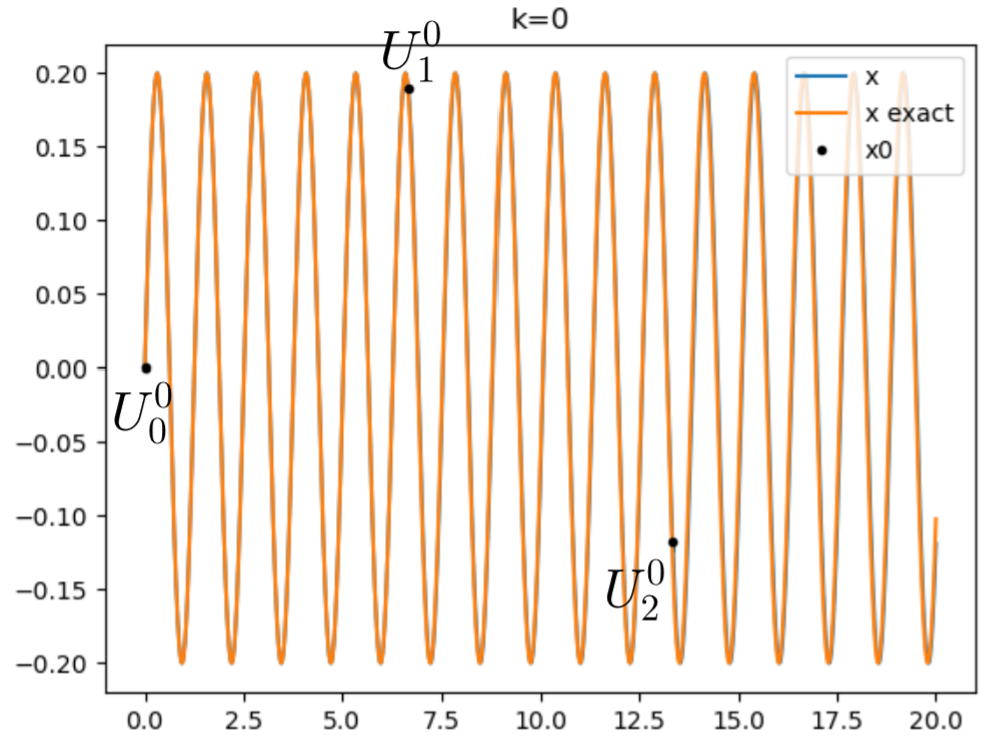
\includegraphics[width=\linewidth]{"images/parareal/osci_sol.png"}
			\caption{Parareal method applied to the harmonic oscillator (with C++)}
		\end{figure}
	\end{minipage} \; \qquad
	\begin{minipage}{0.45\linewidth}
		\begin{figure}
			\centering
			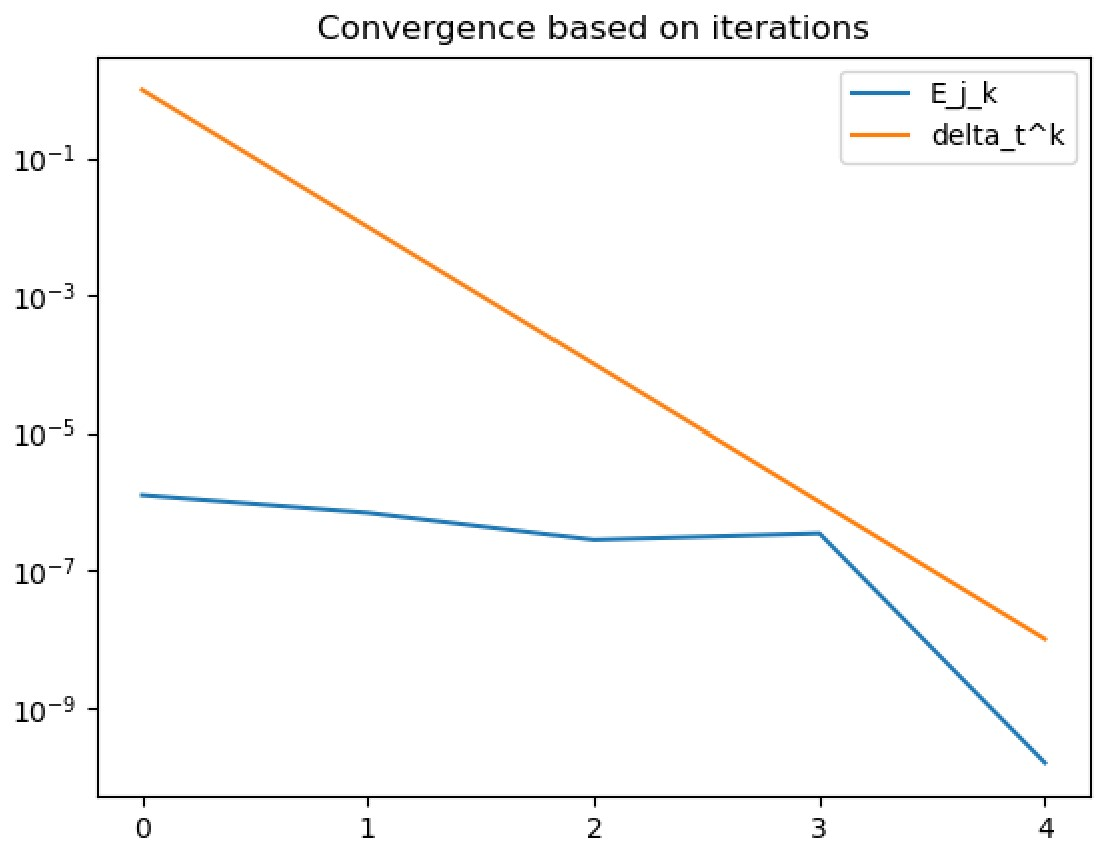
\includegraphics[width=\linewidth]{"images/parareal/osci_cvg_1.jpg"}
			\caption{Convergence property of parareal method with the harmonic oscillator (with Python)}
		\end{figure}
	\end{minipage}
	
\end{frame}

\begin{frame}{Efficiency for the Harmonic oscillator}
	\begin{figure}
		\centering
		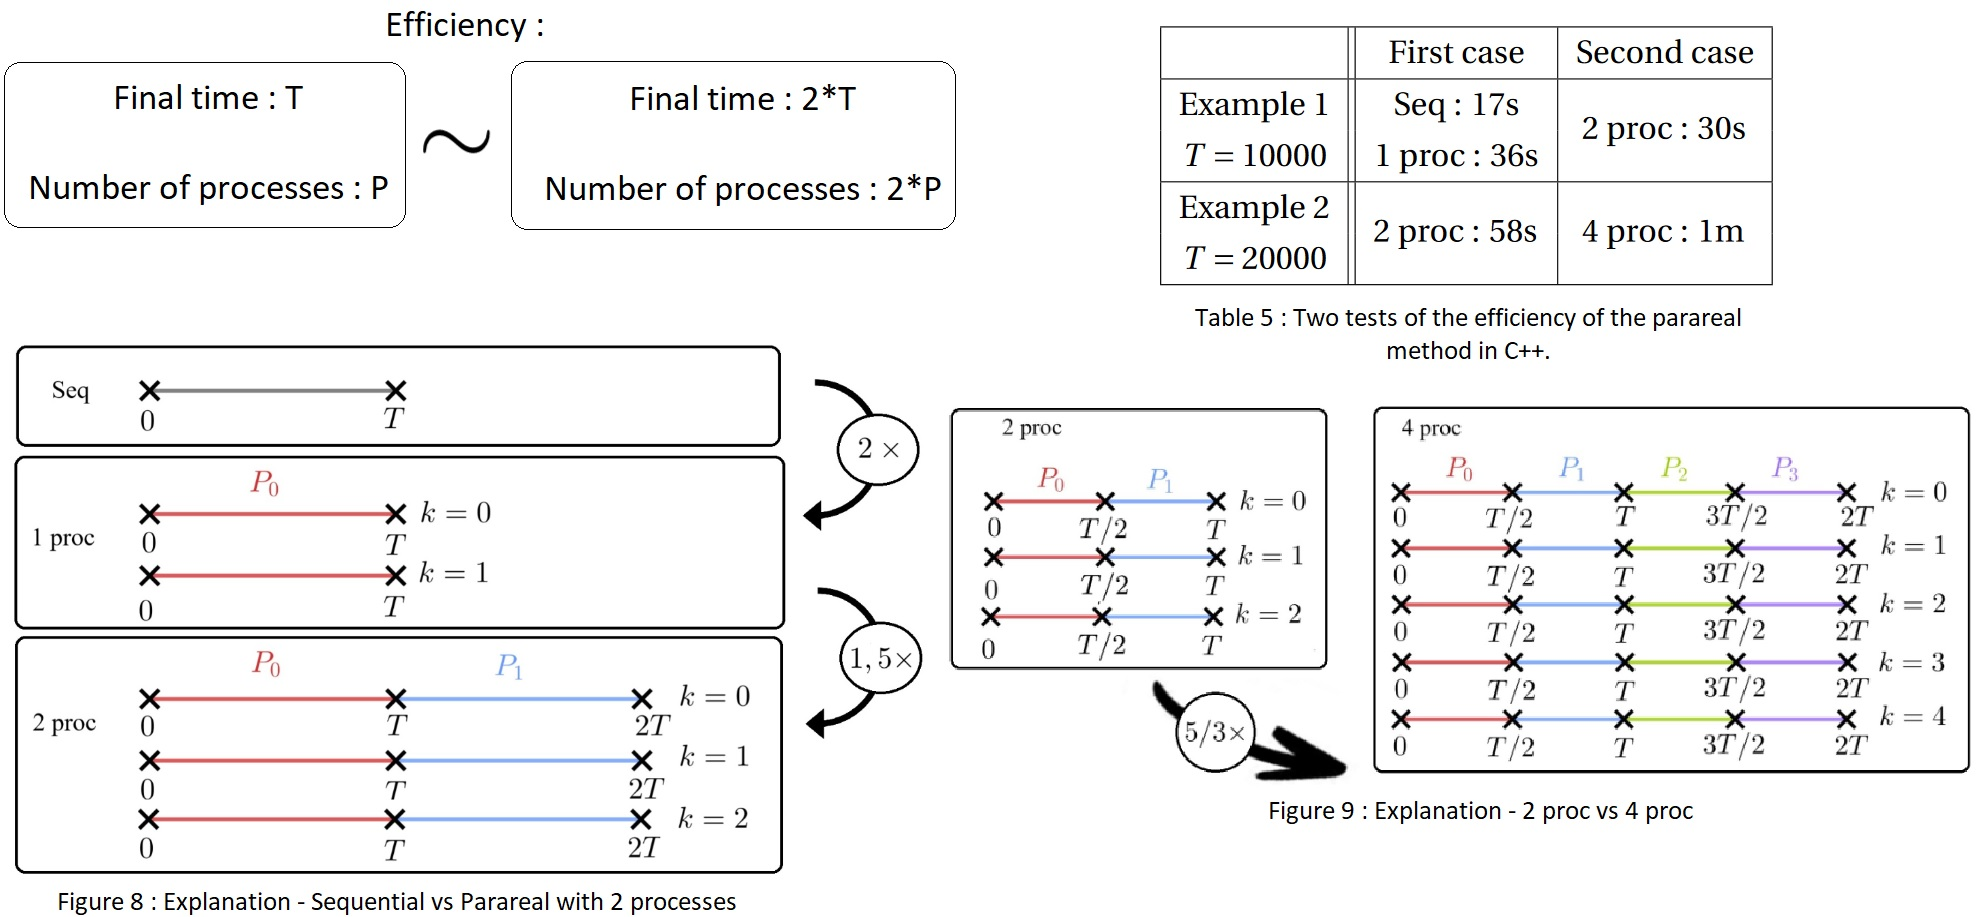
\includegraphics[width=\linewidth]{"images/parareal/efficiency.jpg"}
	\end{figure}
	+ sequential part + operations + communications
\end{frame}

\subsection{Solving PDEs with Feel++}

\begin{frame}{Heat conduction equation}
	
	\textbf{Goal : } apply the parareal method to the resolution of the heat equation using Feel++ (solver developed by Cemosis that uses the finite element method) \\ \; \\
	
	\textbf{The problem :} \\
	We study the heat equation without the convection term and with $\rho=C_p=k=1$
	$$\left\{\begin{aligned}
		\frac{\partial u}{\partial t}-\Delta u &= f \quad&&(t_0,T)\times\Omega \\
		u&=0 \quad&&(t_0,T)\times\partial\Omega\\
		u&=u_0 \quad &&\{0\}\times\Omega
	\end{aligned}\right.$$

	It describes the time evolution of the temperature $u$ of a medium contained in $\Omega$ under an external heat source $f$; $u_0$ is the initial temperature.
	
\end{frame}

\begin{frame}{Laplacian equation}
	
	\begin{minipage}{0.48\linewidth}
		\textbf{The problem :}
		$$\left\{\begin{aligned}
			-\Delta u &= f \quad&&\Omega \\
			u&=g \quad&&\Gamma_D \\
			\frac{\partial u}{\partial n} &=h \quad &&\Gamma_N \\
			\frac{\partial u}{\partial n}+u &=l \quad &&\Gamma_R \\
		\end{aligned}\right.$$
	\end{minipage}
	\begin{minipage}{0.48\linewidth}
		\begin{figure}
			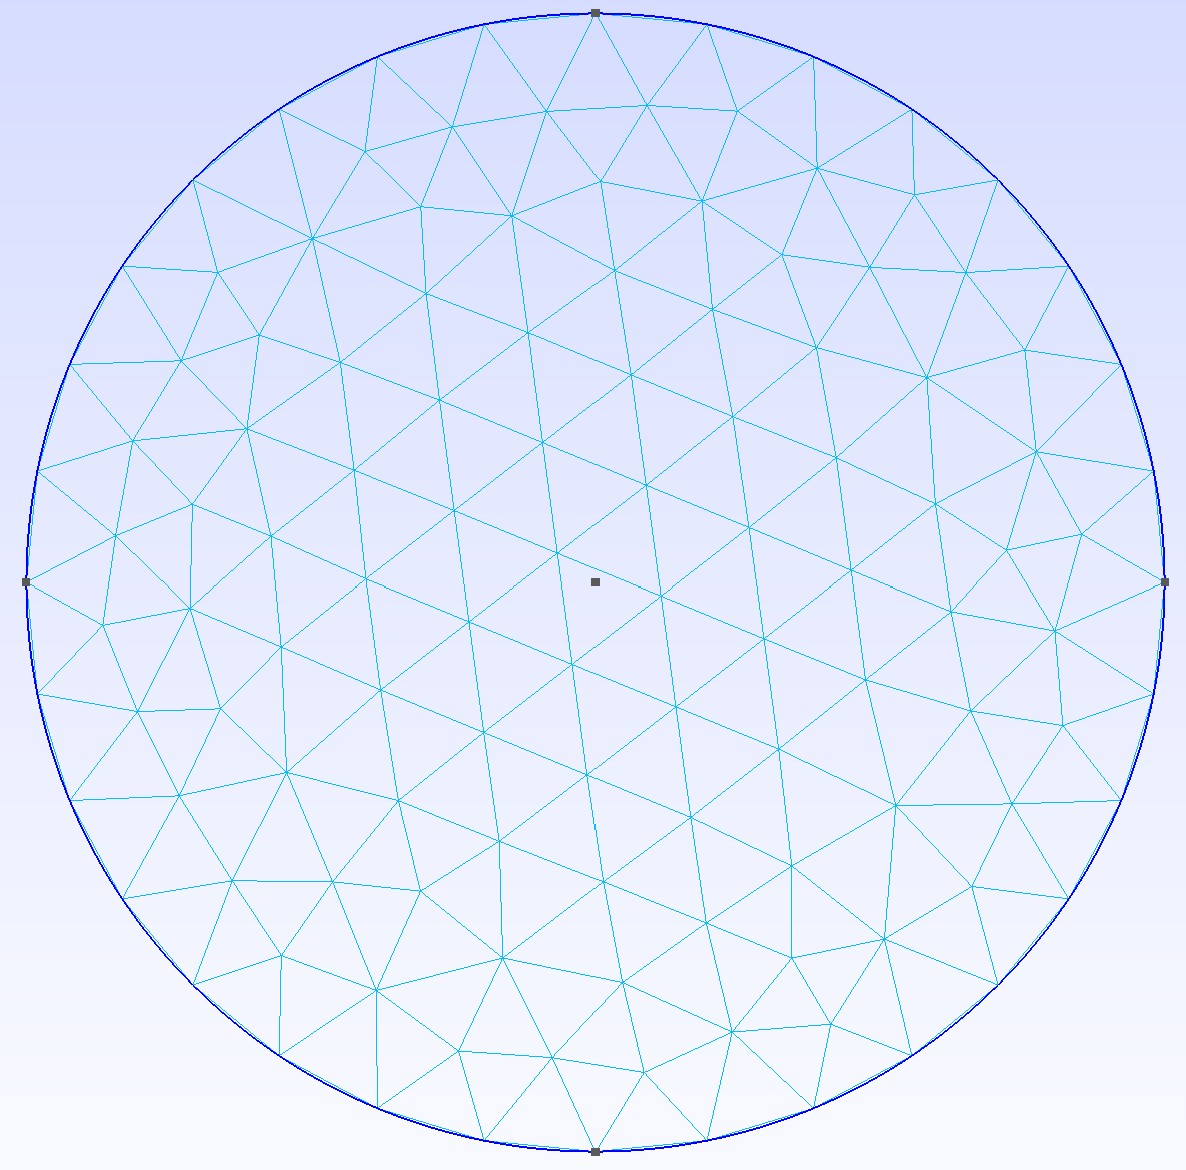
\includegraphics[width=0.8\linewidth]{"images/parareal/circle_mesh.jpg"}
		\end{figure}
	\end{minipage}
	
	\textbf{Weak formulation :} \\
	Find $\; u:\Omega \mapsto \mathbb{R} \;$ such that $\; u\in H_{g,\Gamma_D}^1(\Omega) \;$ and
	$$\int_\Omega \nabla u \cdot \nabla v + \int_{\Gamma_R}uv = \int_\Omega fv + \int_{\Gamma_N}hv+\int_{\Gamma_R}lv \quad \forall v\in H_{0,\Gamma_D}^1(\Omega)$$
	
\end{frame}

\begin{frame}[allowframebreaks]{Convergence with Laplacian}
	\begin{figure}
		\centering
		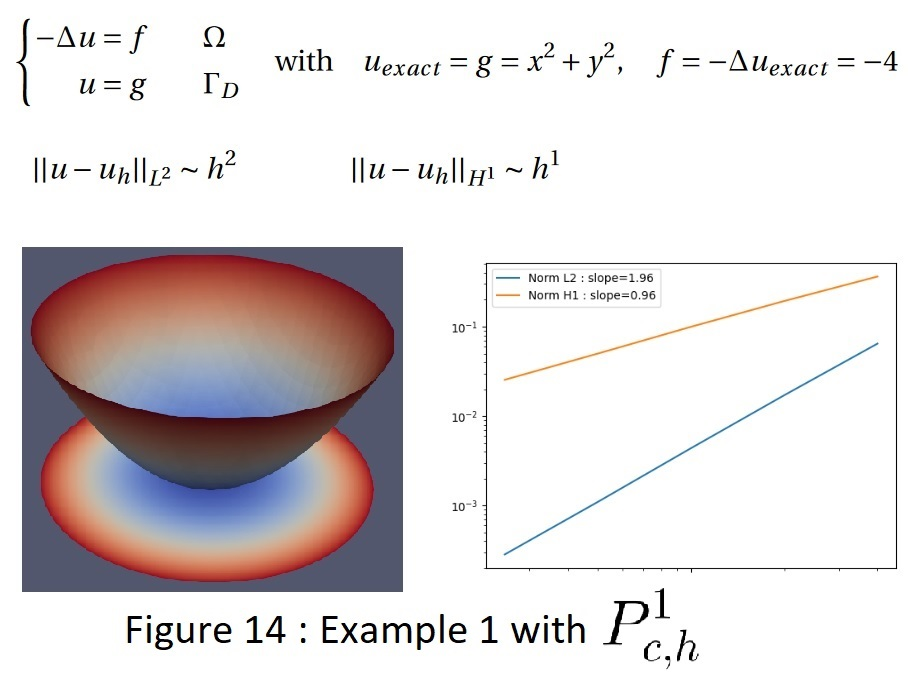
\includegraphics[width=0.7\linewidth]{"images/parareal/convergence_laplace.jpg"}
	\end{figure}

	\newpage
	
	\begin{figure}
		\centering
		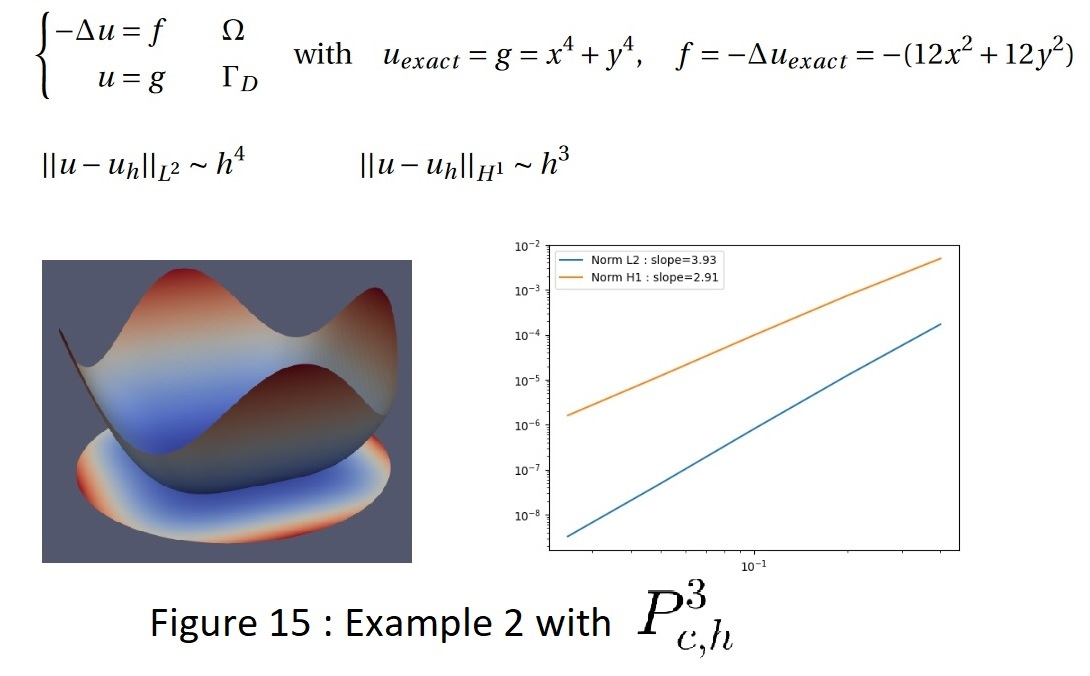
\includegraphics[width=0.8\linewidth]{"images/parareal/convergence_laplace_2.jpg"}
	\end{figure}
\end{frame}

\begin{frame}{Back to the heat equation}
	\textbf{Weak formulation :} \\
	Find $\; u:(t_0,T)\times\Omega \mapsto \mathbb{R} \;$ such that $\; u(t,\cdot)\in H_{g,\Gamma_D}^1(\Omega) \;$ and
	$$\boxed{\int_\Omega \frac{\partial u}{\partial t}(t,x)v(x)dx}+\int_\Omega \nabla u(t,x)\cdot\nabla v(x)dx = \int_\Omega f(t,x)v(x)dx \quad \forall v\in H_{0,\Gamma_D}^1(\Omega)$$
	for almost every $t\in(0,T)$.
	
	\textbf{Temporal discretization :}
	$$\int_\Omega \frac{\partial u}{\partial t}(t,x)v(x)dx \simeq \int_\Omega \frac{u^{n+1}(x)-u^n(x)}{\Delta t}v(x)dx$$
	
	We then obtain :
	$$\frac{1}{\Delta t}\int_\Omega u^{n+1}(x)v(x)dx+\int_\Omega \nabla u^{n+1}(t,x)\cdot\nabla v(x)dx$$
	$$=\int_\Omega f(t,x)v(x)dx + \frac{1}{\Delta t}\int_\Omega u^n(x)v(x)dx$$
\end{frame}

\begin{frame}[allowframebreaks]{Parareal method with the Heat equation}
	\textbf{Provided :} a class \textbf{Heat} allowing the solution of the heat equation with Feel++ (constructor define : the bilinear form $a$ + the linear form $l$ + boundary conditions). \\
	
	\textbf{Test case :}
	\begin{enumerate}[\textbullet]
		\item Spatial : 2 sub-domains.
		\item Temporal : 2 sub-domains, which makes 2*2 processes for the fine integrator and 2 processes for the coarse integrator, so 6 processes in all. We can then run in parallel with 6 processes.
	\end{enumerate}
	\begin{figure}[H]
		\centering
		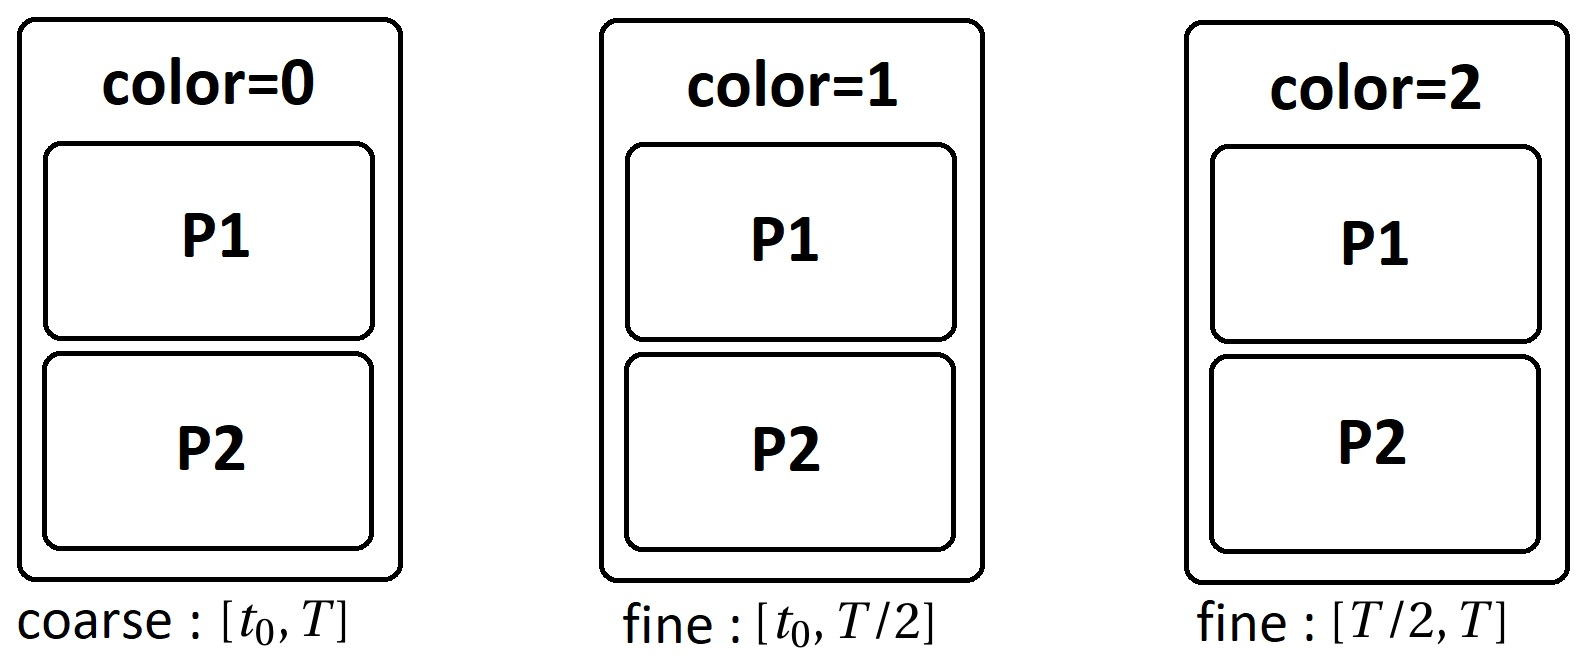
\includegraphics[width=0.5\linewidth]{"images/parareal/master_slave.jpg"}
	\end{figure}

	\newpage

	Need to communicate :
	\begin{figure}[H]
		\centering
		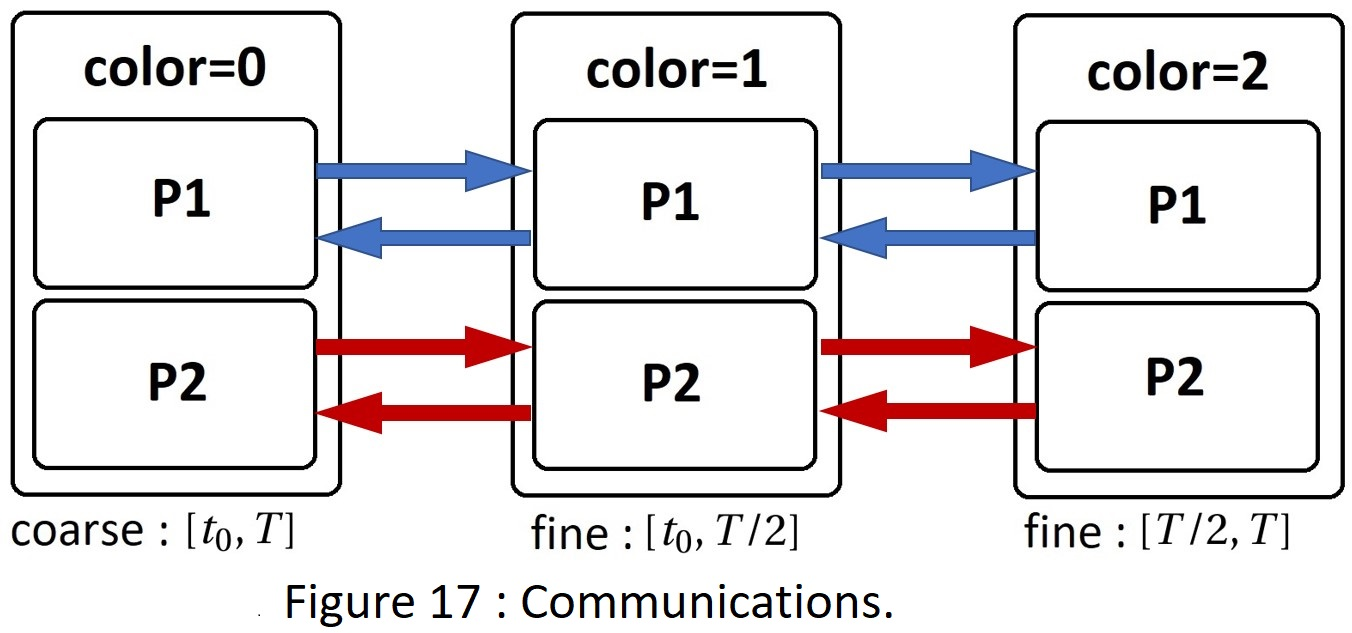
\includegraphics[width=0.45\linewidth]{"images/parareal/master_slave_comm.jpg"}
	\end{figure}
	\begin{figure}[H]
		\centering
		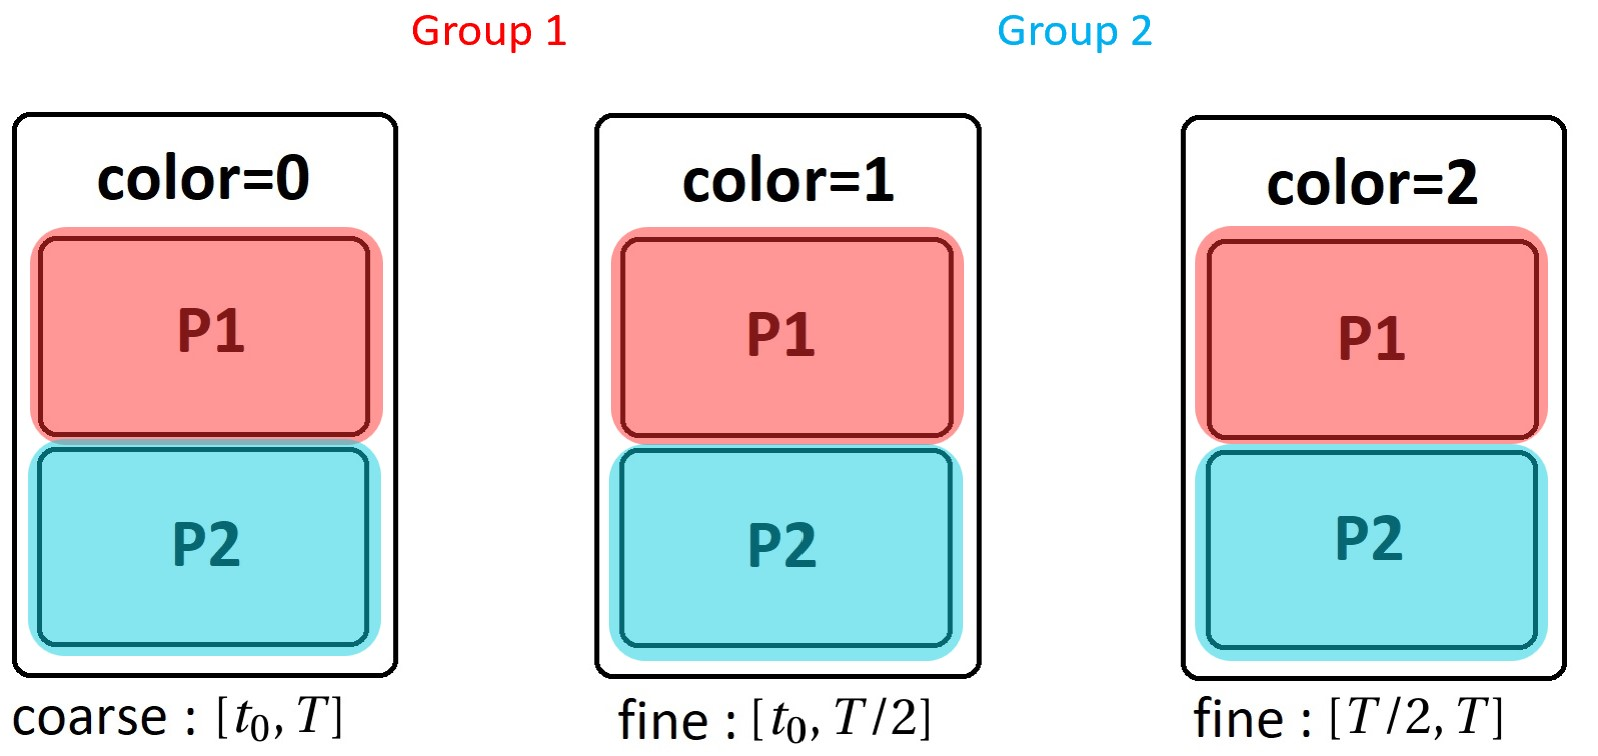
\includegraphics[width=0.45\linewidth]{"images/parareal/master_slave_group.jpg"}
	\end{figure}

	\newpage
	
	Results : Let $t_0=0$, $T=1$ and a piece of finned heat exchanger.
	\begin{figure}[H]
		\centering
		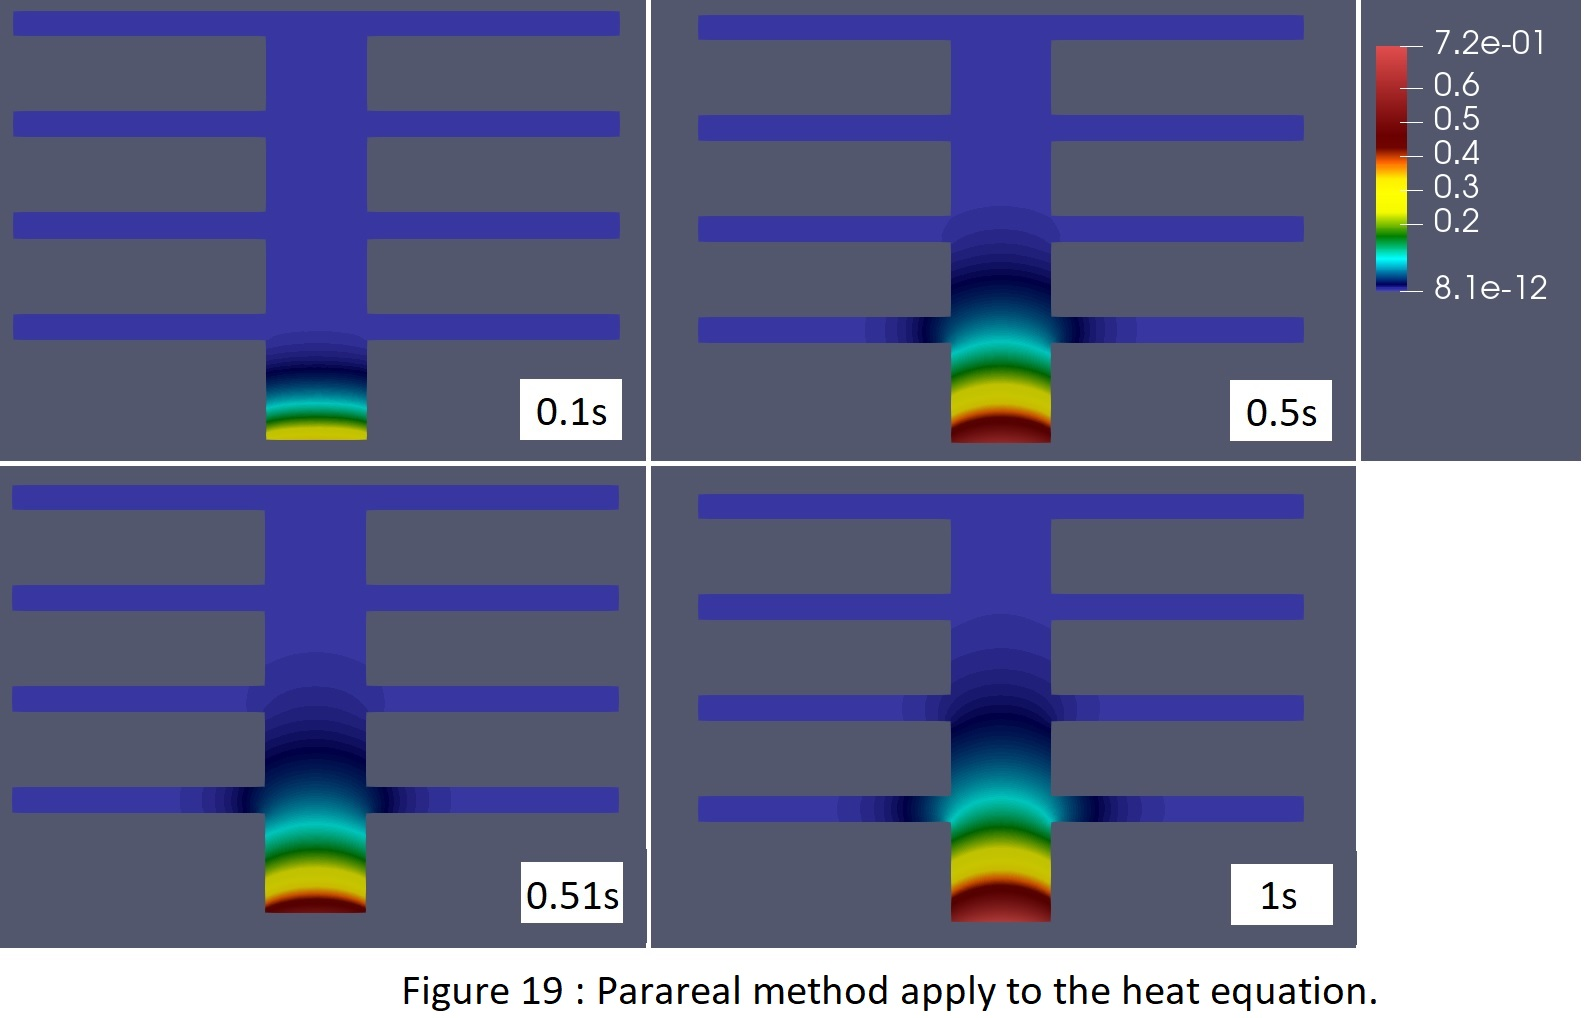
\includegraphics[width=0.7\linewidth]{"images/parareal/heat_results.jpg"}
	\end{figure}
\end{frame}





